% !TEX program = xelatex
% RAI Risk Taxonomy Technical Report 2.0, current release edition.
\documentclass[11pt,a4paper]{article}
\usepackage[a4paper,top=22mm,bottom=24mm,left=22mm,right=22mm]{geometry}
\usepackage{fontspec}
\usepackage{microtype}
\usepackage{booktabs,tabularx,array}
\usepackage{enumitem}
\usepackage{amsmath,amssymb}
\usepackage{seqsplit}
\usepackage{graphicx}
\usepackage{float}
\usepackage{pgfplots}
\usepackage{fancyhdr}
\usepackage[hidelinks]{hyperref}
\pgfplotsset{compat=1.18}

\IfFileExists{/System/Library/Fonts/Menlo.ttc}{%
  \setmainfont{Times New Roman}\setsansfont{Arial}\setmonofont{Menlo}%
  \newfontfamily\krfont{Apple SD Gothic Neo}%
}{%
  \setmainfont{TeX Gyre Termes}\setsansfont{TeX Gyre Heros}\setmonofont{TeX Gyre Cursor}%
  \newfontfamily\krfont{Noto Sans CJK KR}%
}
\newcommand{\ko}[1]{{\krfont #1}}
\newcommand{\code}[1]{\texttt{#1}}
\newcolumntype{Y}{>{\raggedright\arraybackslash}X}
\newcolumntype{L}[1]{>{\raggedright\arraybackslash}p{#1}}
\setlength{\parindent}{1.4em}
\setlength{\parskip}{0pt}
\setlength{\emergencystretch}{2em}

\definecolor{natureblue}{HTML}{0072B2}
\definecolor{naturevermillion}{HTML}{D55E00}
\definecolor{naturegreen}{HTML}{009E73}
\definecolor{naturegrey}{HTML}{6B6B6B}
\pgfplotsset{
  natureaxis/.style={
    axis x line*=bottom,
    axis y line*=left,
    axis line style={black, line width=0.6pt},
    tick align=outside,
    tick style={black, line width=0.5pt},
    tick label style={font=\sffamily\footnotesize, color=black},
    label style={font=\sffamily\small, color=black},
    legend style={draw=none, fill=none, font=\sffamily\footnotesize},
    grid=none,
    clip=false
  }
}

\pagestyle{fancy}
\setlength{\headheight}{14pt}
\fancyhf{}
\lhead{\footnotesize RAI Risk Taxonomy}
\rhead{\footnotesize Technical Report 2.0}
\cfoot{\footnotesize\thepage}
\hypersetup{
  pdftitle={RAI Risk Taxonomy Technical Report 2.0},
  pdfauthor={RAI Risk Taxonomy Project}
}

\begin{document}

\begin{center}
{\LARGE\bfseries RAI Risk Taxonomy 2.0\par}
\vspace{4pt}
{\large Current hierarchy, reproducible mapping, and reliability validation\par}
\vspace{8pt}
{\large RAI Risk Taxonomy Project\par}
\vspace{2pt}
25 July 2026 \,·\, release candidate v2.18.0-rc
\end{center}

\begin{abstract}
\noindent
RAI Risk Taxonomy 2.0 organizes responsible AI risks across General-purpose
AI, Agentic AI, and Physical AI. The current release preserves 1,711 registered
identifiers and distinguishes 1,660 independent active L4 cards from 51 merged
provenance records. A hybrid design combines standards-led hierarchy
construction with literature-derived L4 evidence. The current hierarchy
contains three semantic L2 categories and 54 semantic L3 families. Four
General-purpose AI families were added for societal impact, and nine former
Physical AI societal families were migrated into the shared General-purpose AI
branch. L4 placement uses BGE-M3 embeddings, bilingual L3 definitions,
centroid similarity, direct definition similarity, and keyword similarity under
domain constraints. Reproducibility is supported by fixed inputs, model
snapshot, deterministic seeds, content hashes, iteration traces, and invariant
tests. On 1,660 active cards, seeded spherical EM converges in 20 iterations at
a mean cosine objective of 0.8005. The released L3 appears within the nearest
centroid at Top-1 for 71.9\% of cards and within Top-5 for 95.2\%. These results
establish a reproducible current baseline while preserving human review for
semantically ambiguous cases.
\end{abstract}

\noindent\textbf{Keywords:} AI risk taxonomy; semantic mapping; BGE-M3;
reproducibility; Agentic AI; Physical AI.

\section{Scope and design objective}

AI risk has expanded from text-content harms to autonomous action, tool use,
multi-agent interaction, and direct physical-world effects. RAI Risk Taxonomy
2.0 addresses this broader scope through a five-level structure from L0 to L4.
L1 separates three technological domains. L2 captures the common safety
dimension. L3 defines risk families. L4 records a concrete risk mechanism with
a stable identifier, bilingual label and definition, metrics, and evidence.

The report distinguishes identifiers from active analytical units. The
registry contains 1,711 stable IDs. Of these, 1,660 are independent active
cards and 51 are merged records retained for citation and provenance. All
hierarchy statistics and reliability tests use the 1,660 active cards unless a
table explicitly states otherwise.

\section{Evidence and registry construction}

\subsection{Top-down evidence filter}

The integrated evidence space contains papers, policy reports, and patents.
AI-risk evidence is selected through reviewed risk-source collections,
record-type inclusion rules, valid-title checks, schema standardization, and
within-type deduplication. Evidence records support risk interpretation but do
not map one-to-one onto L4 cards.

\begin{table}[H]
\centering
\caption{Evidence-to-taxonomy stages in the current release.}
\label{tab:funnel}
\small
\begin{tabularx}{\linewidth}{L{0.23\linewidth}r L{0.18\linewidth}Y}
\toprule
Stage & Count & Unit & Inclusion rule \\
\midrule
AI evidence & 3,906,767 & Record & AI source collection, valid title, standardized schema, within-type deduplication \\
AI-risk evidence & 82,971 & Record & Reviewed AI-risk sources and record-type filters \\
Exact-deduplicated candidates & 1,725 & Card candidate & Exact normalized label and core-definition match \\
Registered L4 IDs & 1,711 & Identifier & L3-label leakage removed while identifiers remain auditable \\
Active L4 cards & 1,660 & Independent card & Registry-preserving consolidation excludes 51 merged records from active analysis \\
\bottomrule
\end{tabularx}
\end{table}

\begin{figure}[H]
\centering
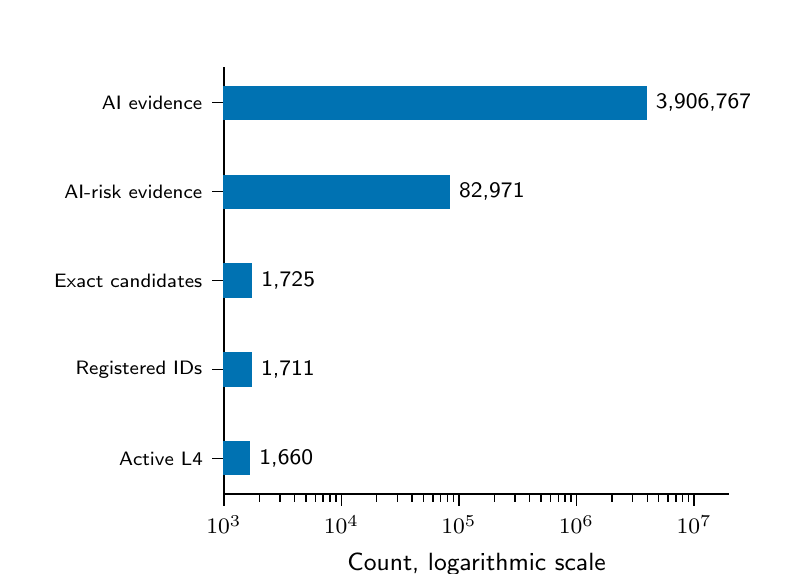
\begin{tikzpicture}
\begin{axis}[
  natureaxis,
  xbar,
  xmode=log,
  log origin=infty,
  log basis x=10,
  xmin=1000,
  xmax=20000000,
  width=0.66\linewidth,
  height=7.0cm,
  xlabel={Count, logarithmic scale},
  symbolic y coords={Active L4,Registered IDs,Exact candidates,AI-risk evidence,AI evidence},
  ytick=data,
  yticklabel style={font=\sffamily\scriptsize,text width=2.1cm,align=right},
  bar width=12pt,
  point meta=explicit symbolic,
  nodes near coords={\pgfplotspointmeta},
  nodes near coords style={font=\sffamily\footnotesize, anchor=west},
]
\addplot[fill=natureblue, draw=natureblue] coordinates {
  (1660,Active L4) [1,660]
  (1711,Registered IDs) [1,711]
  (1725,Exact candidates) [1,725]
  (82971,AI-risk evidence) [82,971]
  (3906767,AI evidence) [3,906,767]
};
\end{axis}
\end{tikzpicture}
\caption{\textbf{Evidence and registry funnel.} The statistical unit changes
from evidence records to risk-card identifiers. Active analysis excludes merged
records without deleting their IDs.}
\label{fig:funnel}
\end{figure}

\subsection{Registry invariants}

The current build enforces four invariants:
\begin{enumerate}[leftmargin=2em]
  \item every registered identifier occurs exactly once;
  \item every merged record points to an active canonical card;
  \item every active card has one operational primary path and one semantic L3 path;
  \item retired or merged records are excluded from active-card metrics.
\end{enumerate}

\section{Current hierarchy}

\subsection{L1 to L3 structure}

The semantic L2 vocabulary is Interaction Safety, System Safety, and Societal
Impact. These categories are instantiated only where a domain has relevant
families. The current hierarchy contains 54 semantic L3 families: 33 General,
6 Agentic, and 15 Physical. Four General societal families were added:
Energy Consumption and Environmental Pollution, Lack of Accountability and
Governance Framework, Lack of Transparency, and Fairness. Nine former Physical
societal families were migrated into General Societal Impact. Existing
similarly named families were retained so that L4 cards could be assigned by
relative semantic fit rather than by label deletion.

\begin{table}[H]
\centering
\caption{Current hierarchy coverage by L1 domain.}
\label{tab:l1}
\begin{tabular}{lrrr}
\toprule
L1 domain & Semantic L3 & Active primary-path L4 & Share of active L4 \\
\midrule
General-purpose AI & 33 & 1,221 & 73.6\% \\
Agentic AI & 6 & 281 & 16.9\% \\
Physical AI & 15 & 158 & 9.5\% \\
\midrule
Total & 54 & 1,660 & 100.0\% \\
\bottomrule
\end{tabular}
\end{table}

The primary-path counts in Table~\ref{tab:l1} describe the deployed navigation
tree. For semantic analysis, cards under review are attributed to their
retained semantic review path. This produces the L1 by L2 distribution in
Table~\ref{tab:l2}. The five-card difference between primary-path and semantic
domain counts arises from cross-domain review paths and does not change the
total.

\begin{table}[H]
\centering
\caption{Active L4 cards by semantic L1 and L2 path.}
\label{tab:l2}
\begin{tabular}{lrrrr}
\toprule
L1 domain & Interaction Safety & System Safety & Societal Impact & Total \\
\midrule
General-purpose AI & 641 & 467 & 108 & 1,216 \\
Agentic AI & 0 & 286 & 0 & 286 \\
Physical AI & 64 & 94 & 0 & 158 \\
\midrule
Total & 705 & 847 & 108 & 1,660 \\
\bottomrule
\end{tabular}
\end{table}

\subsection{Hierarchy coverage}

All 1,660 active cards have a semantic L3 path. All 54 semantic L3 families are
occupied and each contains at least one released card outside the review
subset. Anthropomorphism is the largest family with 160 cards, equal to 9.6\%
of active L4 cards. The five largest families contain 553 cards, or 33.3\%.

\begin{figure}[H]
\centering
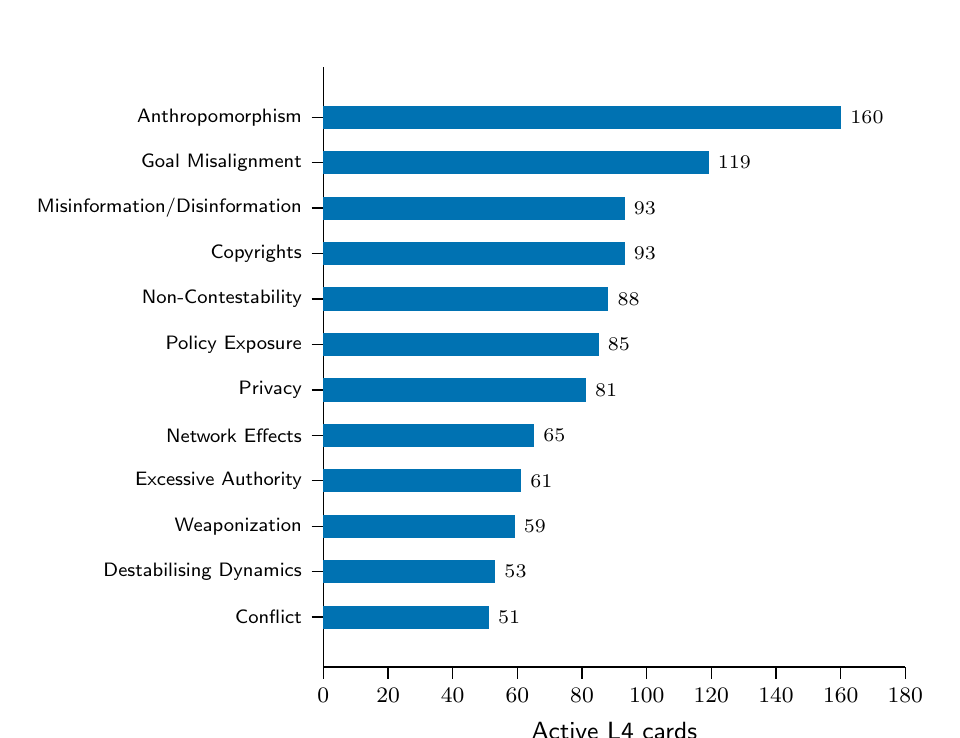
\begin{tikzpicture}
\begin{axis}[
  natureaxis,
  xbar,
  xmin=0,
  xmax=180,
  width=0.74\linewidth,
  height=9.2cm,
  xlabel={Active L4 cards},
  symbolic y coords={Conflict,Destabilising Dynamics,Weaponization,Excessive Authority,Network Effects,Privacy,Policy Exposure,Non-Contestability,Copyrights,Misinformation/Disinformation,Goal Misalignment,Anthropomorphism},
  ytick=data,
  yticklabel style={font=\sffamily\scriptsize},
  bar width=8pt,
  nodes near coords,
  nodes near coords style={font=\sffamily\scriptsize, anchor=west},
]
\addplot[fill=natureblue, draw=natureblue] coordinates {
  (51,Conflict)
  (53,Destabilising Dynamics)
  (59,Weaponization)
  (61,Excessive Authority)
  (65,Network Effects)
  (81,Privacy)
  (85,Policy Exposure)
  (88,Non-Contestability)
  (93,Copyrights)
  (93,Misinformation/Disinformation)
  (119,Goal Misalignment)
  (160,Anthropomorphism)
};
\end{axis}
\end{tikzpicture}
\caption{\textbf{Twelve largest semantic L3 families.} Counts use the retained
semantic path for boundary-review cards and exclude 51 merged records.}
\label{fig:l3}
\end{figure}

\section{Reproducible L4 to L3 mapping}

\subsection{Representations and constraints}

Each active card is represented by the concatenation of its English and Korean
label and definition. Each L3 seed uses the same four fields. BGE-M3 encodes
both card and seed text into normalized 1,024-dimensional vectors. English
TF-IDF vectors provide a complementary keyword signal.

Physical source-card identities remain locked, and their paths are changed only
when an approved revision is imported from the authoritative Physical AI
master. The 31 July 2026 synchronization imported two such revisions after
24-condition EM sensitivity testing and 1,000 bootstrap repeats.
General cards can compete across General families. Agentic candidates require
an explicit autonomous execution mechanism unless the source card is already
Agentic. The migrated societal families compete inside the General branch.
These constraints prevent generic vocabulary from moving cards into a
technology-specific domain.

\subsection{Iterative winner assignment}

For card $i$ and candidate family $k$, the mapping score is
\begin{equation}
S_{ik}
=0.60\cos(x_i,\mu_k)
+0.30\cos(x_i,s_k)
+0.10\cos(t_i,q_k),
\end{equation}
where $x_i$ is the normalized BGE-M3 card embedding, $\mu_k$ is the current
family centroid, $s_k$ is the bilingual L3 seed embedding, and $t_i$ and $q_k$
are TF-IDF representations. Centroids are updated from assigned members,
definition seeds, and approved prior members:
\begin{equation}
\mu_k \leftarrow
\operatorname{norm}
\left(0.75\bar{x}_k+0.15s_k+0.10\bar{x}^{\,prior}_k\right).
\end{equation}
When no prior member set exists, the member and seed weights are 0.85 and 0.15.
The constrained winner is accepted only when it improves the current score by
the configured margin. The release build reached a fixed point after four
mapping iterations, with 144, 13, 5, and 0 changed cards. In total, 182 active
cards received a structural or competitive path update, including 30 societal
structure migrations.

\subsection{Boundary-review status}

The review marker is metadata on a semantic assignment, not a separate risk
concept. It is retained when a proposed placement does not jointly satisfy a
direct seed cosine of at least 0.45 and a composite-score margin of at least
0.015, or when the card lies outside the approved extension scope. The current
release resolves 151 prior review markers and retains 614 cards for subsequent
human adjudication. This status is reported only as a quality-control boundary
and is not counted as an L2 or L3 family.

\section{Reliability validation}

\subsection{Validation design}

The released semantic path is evaluated against centroids formed from the
released assignments. Three diagnostics are used:
\begin{enumerate}[leftmargin=2em]
  \item \textbf{EM convergence}: seeded spherical EM repeatedly updates
  centroids and assignments until no assignment changes.
  \item \textbf{Top-$k$ containment}: the share of cards whose released L3
  appears among the $k$ nearest released-family centroids.
  \item \textbf{Perturbation stability}: agreement between unperturbed and
  perturbed nearest-centroid assignments after Gaussian noise is added to
  normalized embeddings.
\end{enumerate}

The validation uses seed 20260723, 5,000 label permutations, and 200
perturbation repeats at each noise level. All 54 L3 seed rows are retained in
both evaluated populations. The released subset excludes 614 boundary-review
cards but does not refit or reduce the L3 vocabulary.

\begin{table}[H]
\centering
\caption{Current reliability results at v2.18.0-rc.}
\label{tab:validation}
\small
\begin{tabular}{lrr}
\toprule
Diagnostic & All active cards & Released subset \\
\midrule
Cards assessed & 1,660 & 1,046 \\
Semantic L3 families & 54 & 54 \\
EM iterations to fixed point & 20 & 12 \\
Final mean cosine objective & 0.8005 & 0.8026 \\
Top-1 containment & 71.9\% & 81.6\% \\
Top-2 containment & 85.3\% & 91.2\% \\
Top-3 containment & 91.3\% & 94.6\% \\
Top-5 containment & 95.2\% & 97.2\% \\
Median assignment margin & 0.0168 & 0.0310 \\
Negative-margin share & 28.1\% & 18.4\% \\
Permutation $p$ & 0.0002 & 0.0002 \\
Stability at $\sigma=0.01$ & 95.0\% & 96.0\% \\
Stability at $\sigma=0.05$ & 75.0\% & 80.7\% \\
\bottomrule
\end{tabular}
\end{table}

\begin{figure}[H]
\centering
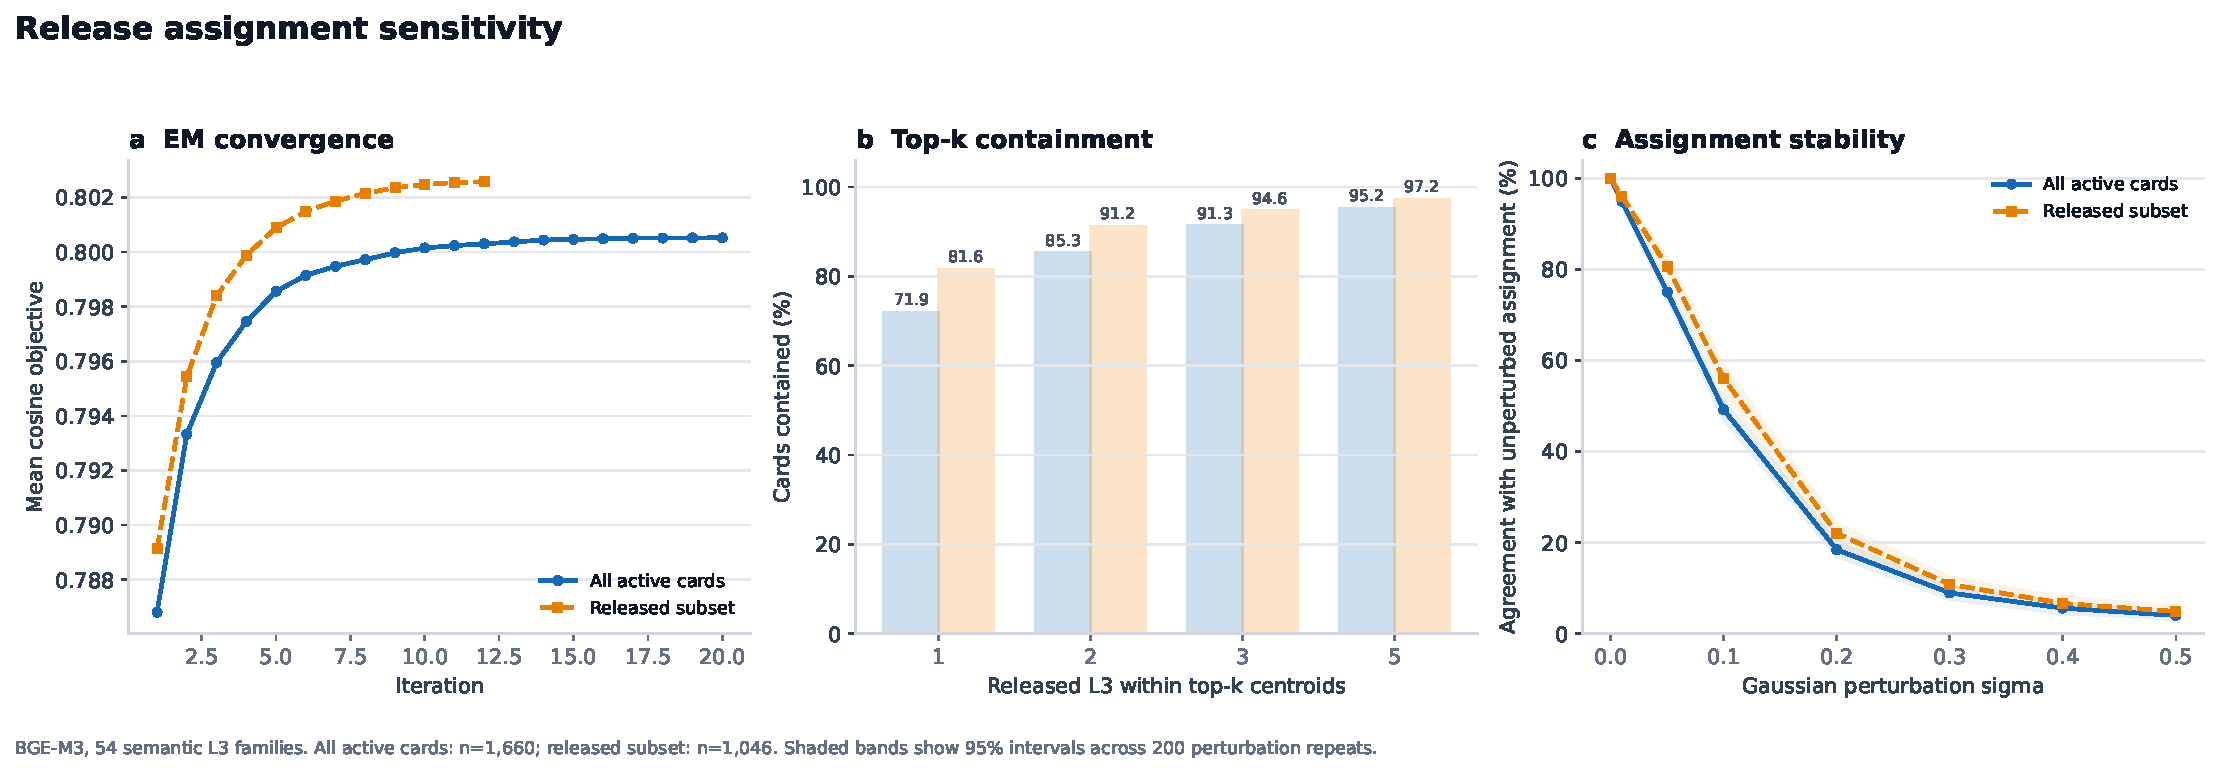
\includegraphics[width=\textwidth]{../validation/v2.18.0-rc/hold_sensitivity_bge_m3/release_assignment_sensitivity_3panel.pdf}
\caption{\textbf{Sensitivity diagnostics for all active cards and the released
subset.} Panels show seeded spherical-EM convergence, Top-$k$ containment, and
assignment stability under Gaussian perturbation. Shaded bands are 95\%
intervals across 200 repeats.}
\label{fig:sensitivity}
\end{figure}

The higher containment and perturbation stability of the released subset show
that the quality-control boundary separates a less stable region of the
semantic space. This comparison does not prove that every released assignment
is correct. It provides a reproducible prioritization signal for human review.

\section{Granularity-flow tiers}

\subsection{Measured merge boundary}

Leaf-level granularity is fixed by a merge threshold on the cosine-similarity
graph of card embeddings, where connected components are merge clusters. Rather
than fixing that threshold by analyst judgment, the release derives it from the
inventory. For a candidate threshold $\tau$, let $\Phi_{\mathrm{coh}}(\tau)$ be
the pooled within-cluster mean similarity and $\Phi_{\mathrm{att}}(\tau)$ the
mean over clusters of the maximum similarity to any card outside the cluster.
The operating boundary is the smallest $\tau$ at which cohesion still dominates
attraction,
\[
\tau^{*}=\min\{\tau:\Phi_{\mathrm{coh}}(\tau)\ge\Phi_{\mathrm{att}}(\tau)\},
\]
evaluated on a $10^{-4}$ grid. On the normalized master inventory of 1,612
active cards, $\tau^{*}=0.8329$.

\subsection{Iterated consolidation}

Merging at $\tau^{*}$ changes the density of the space, so the boundary moves
with it. Repeating the cycle of merge, re-derive, and merge again generates a
sequence of boundaries and inventories, the granularity flow. Each step is
scored against a size-matched random-group null drawn on its own inventory;
a step is admissible when at least 90\% of its merge groups exceed the null by
two standard deviations. Steps 1 to 5, the range released for review, satisfy
this rule with a fraction of 1.00 throughout and a median $z$ between 3.27 and
4.30. Representatives are medoids of their merge group, so every tier card is
an original card rather than a synthesized summary.

\begin{table}[H]
\centering
\caption{Granularity-flow tiers. Merge groups are counted per consolidation step
and absorbed cards cumulatively from the Master inventory. Domain counts follow
the L3 re-assignment, with the Societal Safety axis routed by scope.}
\label{tab:ftiers}
\small
\begin{tabularx}{\linewidth}{lrrrrY}
\toprule
Tier & $\tau^{*}$ & Cards & Merge groups & Absorbed & General / Agentic / Physical \\
\midrule
Master & --     & 1,612 & --  & --  & 1,154 / 155 / 303 \\
F1     & 0.8329 & 1,383 & 109 & 229 & 906 / 140 / 337 \\
F2     & 0.8033 & 1,154 & 121 & 458 & 734 / 128 / 292 \\
F3     & 0.7903 & 1,038 & 81  & 574 & 653 / 112 / 273 \\
F4     & 0.7753 & 901   & 82  & 711 & 568 / 92 / 241 \\
F5     & 0.7634 & 792   & 70  & 820 & 491 / 83 / 218 \\
\bottomrule
\end{tabularx}
\end{table}

Societal Safety is a single concept family applied at three scopes rather than a
General-only axis. Its L3 nodes therefore branch as
\texttt{RAI3-\{G$\vert$A$\vert$P\}-SOC-nn}, where a given \texttt{nn} denotes the
same risk concept at each scope; L4 identifiers are unchanged and only the owning
L3 branches. A card is Physical when its label or definition carries a physical
referent such as a robot, embodiment, hardware, sensor or product-safety
grounding; Agentic when it is not Physical but binds to agent autonomy, long
horizon goals, tool use or multi-agent interaction; and General otherwise. On the
Master inventory the 430 Societal Safety cards split 351 General, 37 Agentic and
42 Physical, and the tier counts above follow that routing.

\subsection{Cross-corpus replication}

To test whether the procedure depends on this particular inventory, the same
pipeline was applied without retuning to the MIT AI Risk Repository, whose risk
categories and subcategories were embedded with the same encoder. The
replication reproduces both the two transitions and the crossing, and the flow
behaves as it does here.

\begin{table}[H]
\centering
\caption{Granularity flow on the MIT AI Risk Repository. Merge groups and median
$z$ are per consolidation step; absorbed entries are cumulative. Domain columns
are omitted because that repository uses its own top-level scheme.}
\label{tab:mittiers}
\small
\begin{tabularx}{\linewidth}{lrrrrrY}
\toprule
Tier & $\tau^{*}$ & Entries & Merge groups & Absorbed & Median $z$ & Role \\
\midrule
Source & --     & 1,810 & --  & --    & --   & repository inventory \\
M1     & 0.8190 & 1,423 & 189 & 387   & 4.79 & fidelity tier (crossing) \\
M2     & 0.7908 & 1,230 & 104 & 580   & 3.68 & second consolidation \\
M3     & 0.7696 & 1,022 & 115 & 788   & 3.53 & third consolidation \\
M4     & 0.7545 & 879   & 87  & 931   & 3.17 & compression tier \\
M5     & 0.7374 & 727   & 99  & 1,083 & 3.00 & extended compression tier \\
\bottomrule
\end{tabularx}
\end{table}

Every step clears the validity rule, with at least 98.9\% of merge groups
exceeding the size-matched random-group null by two standard deviations. The
replication is reported for reference and is not released for human audit.

\subsection{Released tiers}

F1, F4, and F5 are released for human audit. F1 preserves the fidelity of the
original inventory at the measured boundary, F4 is the compression tier reached
after four consolidations, and F5 extends compression by one further step. Each
tier is published as a browsable audit page in which every card is judged on
description adequacy, L3 mapping, and redundancy against other cards.

\section{Reproducibility controls}

\subsection{Fixed computational specification}

\begin{table}[H]
\centering
\caption{Reproducibility specification.}
\label{tab:repro}
\small
\begin{tabularx}{\linewidth}{L{0.27\linewidth}Y}
\toprule
Component & Fixed specification \\
\midrule
Release & v2.18.0-rc, derived from sealed v2.17.2 inputs \\
Encoder & BAAI/bge-m3, normalized 1,024-dimensional embeddings \\
Mapping seed & 20260725 \\
Validation seed & 20260723 \\
Maximum mapping iterations & 30, early stop at zero changed assignments \\
Permutation test & 5,000 matched label permutations \\
Perturbation test & 200 repeats for $\sigma\in\{0,0.01,0.05,0.10,0.20,0.30,0.40,0.50\}$ \\
Card input hash & \texttt{\seqsplit{dff3f3269a1ed8575f409923ca0c3db1aca14931259b567abeefa12da2229acf}} \\
Hierarchy input hash & \texttt{\seqsplit{76156ee383cbbf84870989f2036f0a1de6f031308fd0b9f9d5f4b821f0450050}} \\
Card-embedding hash & \texttt{\seqsplit{8f99380ef026730105624d5103a37fea20ceb4816d2c5cace33b2e8c764c19d8}} \\
L3-seed hash & \texttt{\seqsplit{5ead12763d624a8e6d92dbb82536e18710d66c1670107c1d7d3c6e2ff18f6615}} \\
\bottomrule
\end{tabularx}
\end{table}

\subsection{Executable checks}

The release build records the complete hierarchy migration, changed-card list,
iteration trace, threshold decisions, and content hashes. Automated checks
verify the 1,711-ID registry, 1,660 active cards, 51 merged records, 54 semantic
L3 families, domain counts, review-marker count, semantic-space node count,
and absence of dangling paths. Browser smoke tests cover the taxonomy explorer
and semantic-space views. PDF compilation is followed by page rendering and
visual inspection.

A reproduction is accepted only when the following outputs agree:
\begin{enumerate}[leftmargin=2em]
  \item registry and active-card counts;
  \item L1, L2, and L3 totals;
  \item card and hierarchy hashes;
  \item EM fixed-point iterations and final objective;
  \item Top-$k$ and perturbation metrics within the stated rounding rule.
\end{enumerate}

\section{Interpretation and limitations}

The taxonomy is a policy-guided semantic partition, not an unsupervised claim
that each risk has only one natural parent. Some L4 cards contain multiple
mechanisms and can be close to several L3 families. Top-$k$ containment is
therefore reported alongside Top-1. The BGE-M3 geometry measures semantic
proximity, not causal propagation, likelihood, or severity. Locked Physical
paths provide a stable reference but are not an unbiased prediction set.
Human evaluation remains necessary for boundary cases, newly introduced
societal families, and cards affected by structural migration.

\section{Conclusion}

The corrected current hierarchy consists of 1,711 registered IDs, 1,660 active
L4 cards, three semantic L2 categories, and 54 semantic L3 families. Its L3
composition is 33 General, 6 Agentic, and 15 Physical. Section-level tables and
figures use the same active-card snapshot and explicitly distinguish primary
navigation paths from retained semantic review paths. The mapping and
validation workflow is reproducible from fixed model inputs, deterministic
seeds, content hashes, iteration traces, and invariant tests. The current
results provide a defensible baseline for human evaluation and subsequent
release decisions without treating semantic similarity as ground truth.

\section*{References}

\begin{enumerate}[leftmargin=2em]
  \item NIST. \textit{Artificial Intelligence Risk Management Framework
  (AI RMF 1.0)}. 2023.
  \item ISO/IEC. \textit{ISO/IEC 23894:2023 Information technology,
  Artificial intelligence, Guidance on risk management}. 2023.
  \item OWASP. \textit{Top 10 for Large Language Model Applications} and
  \textit{Agentic AI Threats and Mitigations}. Current reviewed editions.
  \item MIT FutureTech. \textit{AI Risk Repository}. Current reviewed release.
  \item BAAI. \textit{BGE-M3: Multi-Lingual, Multi-Functionality,
  Multi-Granularity Text Embeddings}. 2024.
\end{enumerate}

\end{document}
